
	%---------------------------------------------------------------------------------------------------%
	%%%%                                         SUB SECTION                                         %%%%
	%---------------------------------------------------------------------------------------------------%
	\section*{작성 CODE capture}
    \vspace{-2mm}
	Project0과 동일하게, WSL2를 이용해 ubuntu를 구동하면서, Visual Studio Code 의 Remote Shell을 이용한 
	리눅스 실습환경을 구성하였다.
	\vspace{-6mm}
	\subsection*{CLIENT : mySender.c}
%------------------------------------------------------------------------------------------------------이미지
\vspace{-2mm}
	\begin{figure}[!h]
		\centering
			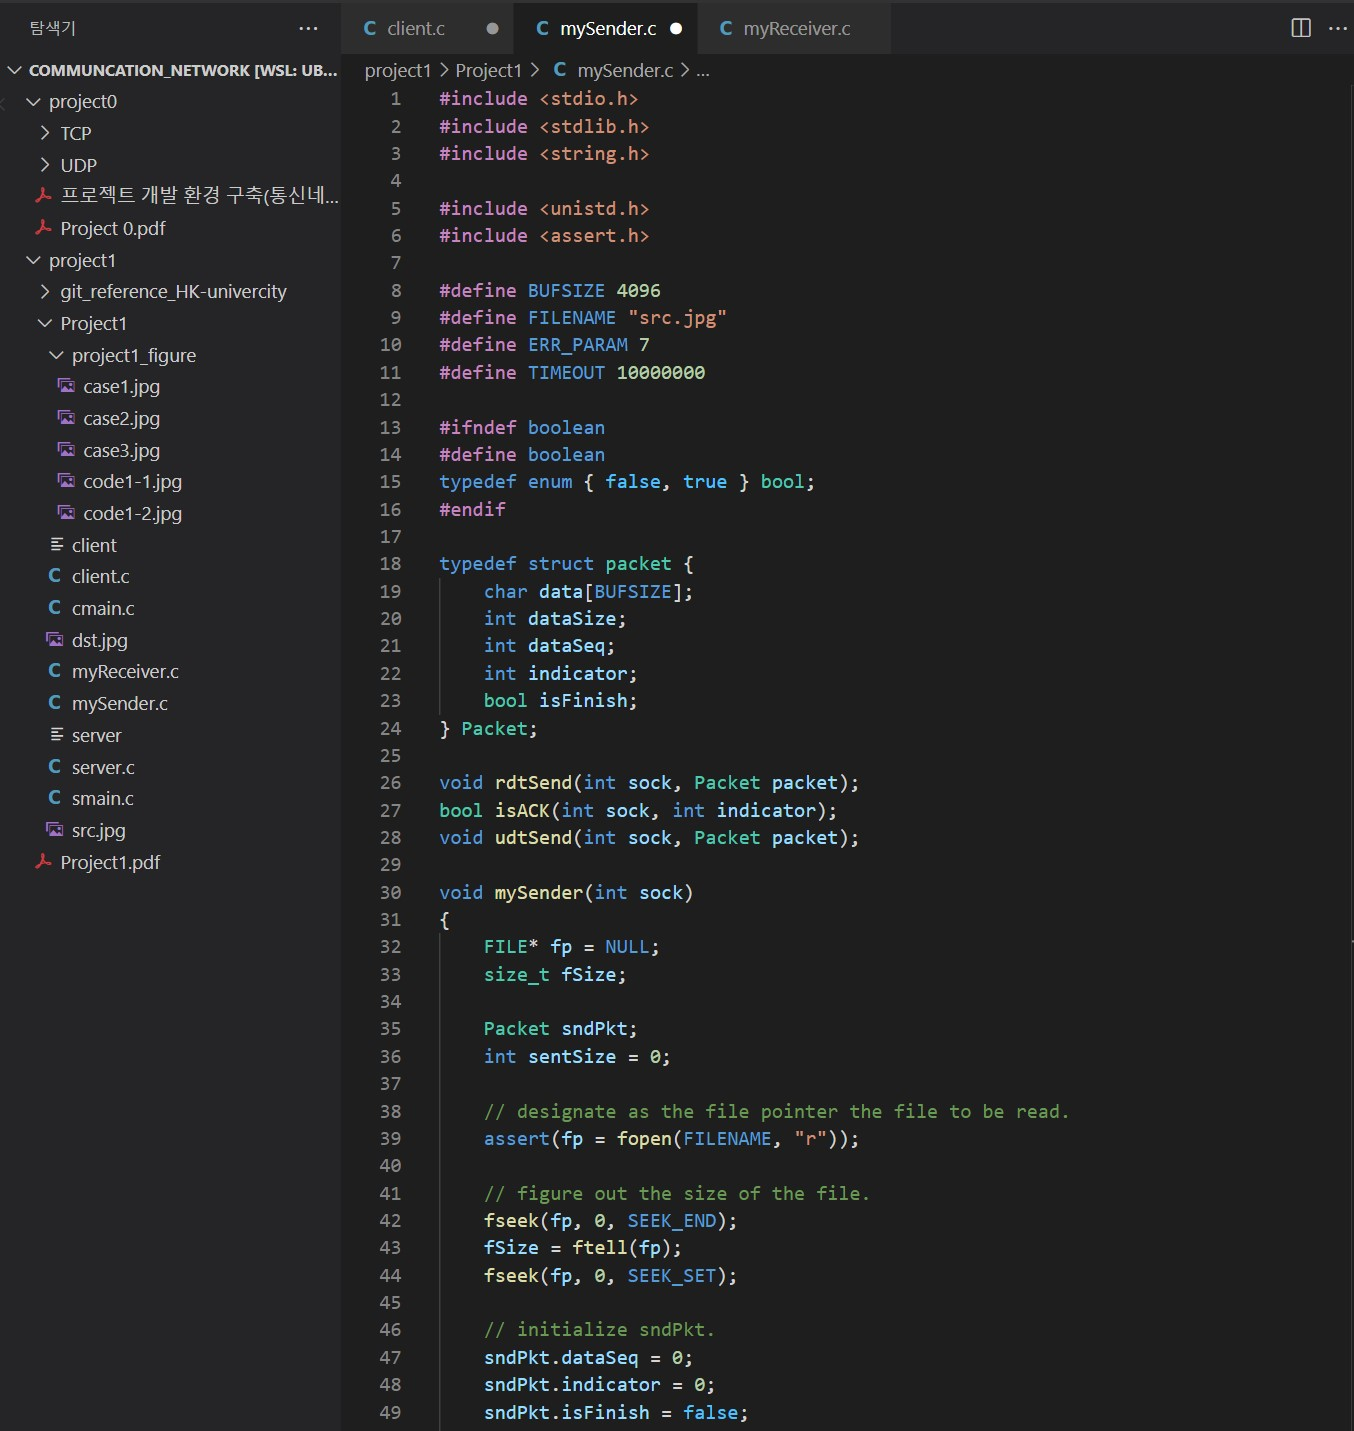
\includegraphics[width=.9\textwidth]{image/code1-1.jpg}
	\end{figure}
\vspace{-8mm}
%------------------------------------------------------------------------------------------------------------
%%%%%%%%%%%%%%%%%%%%%%%%%%%%%%%%%%%%%%%%%%%%%%%%%%%%%%%%%%%%%%%%%%%%%%%%%%%%%%%%%%%%%%%%%%%%%%%%%%%%%
\newpage
%%%%%%%%%%%%%%%%%%%%%%%%%%%%%%%%%%%%%%%%%%%%%%%%%%%%%%%%%%%%%%%%%%%%%%%%%%%%%%%%%%%%%%%%%%%%%%%%%%%%%
%------------------------------------------------------------------------------------------------------이미지
\vspace{0mm}
	\begin{figure}[!h]
		\centering
			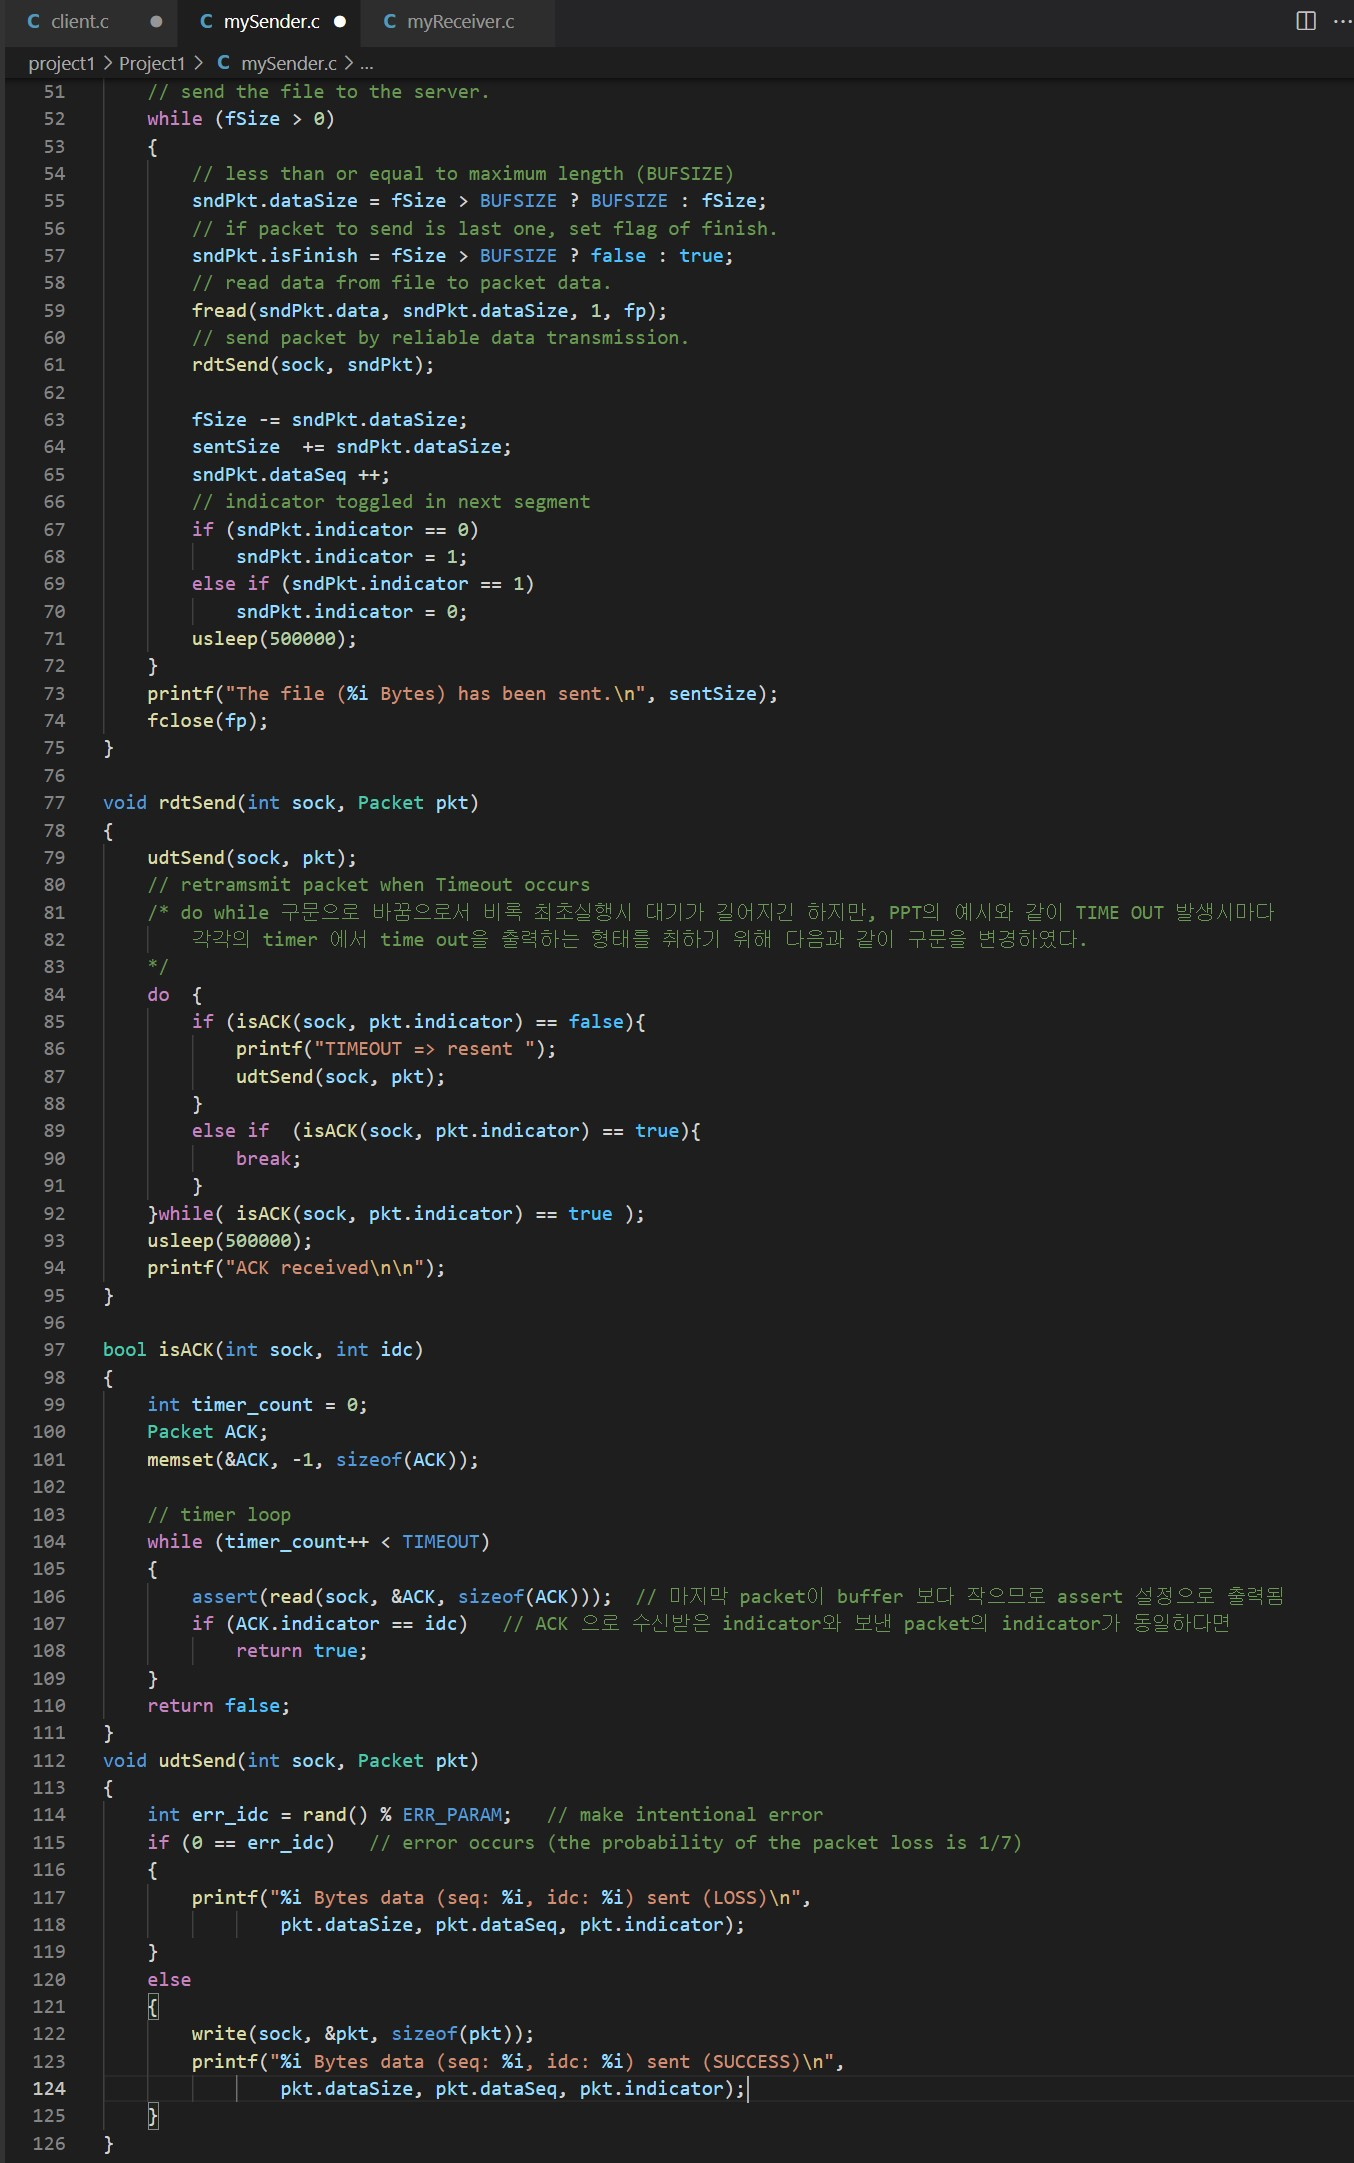
\includegraphics[width=.9\textwidth]{image/code1-2.jpg}
			\caption{rdt 3.0 TCP client's CODE - mySender.c}
	\end{figure}
\vspace{-8mm}
%------------------------------------------------------------------------------------------------------------
%%%%%%%%%%%%%%%%%%%%%%%%%%%%%%%%%%%%%%%%%%%%%%%%%%%%%%%%%%%%%%%%%%%%%%%%%%%%%%%%%%%%%%%%%%%%%%%%%%%%%
\newpage
%%%%%%%%%%%%%%%%%%%%%%%%%%%%%%%%%%%%%%%%%%%%%%%%%%%%%%%%%%%%%%%%%%%%%%%%%%%%%%%%%%%%%%%%%%%%%%%%%%%%%
	%---------------------------------------------------------------------------------------------------%
	%%%%                                         SUB SECTION                                         %%%%
	%---------------------------------------------------------------------------------------------------%
	\subsection*{SERVER : myReceiver.c}
%------------------------------------------------------------------------------------------------------이미지
\vspace{-2mm}
	\begin{figure}[!h]
		\centering
			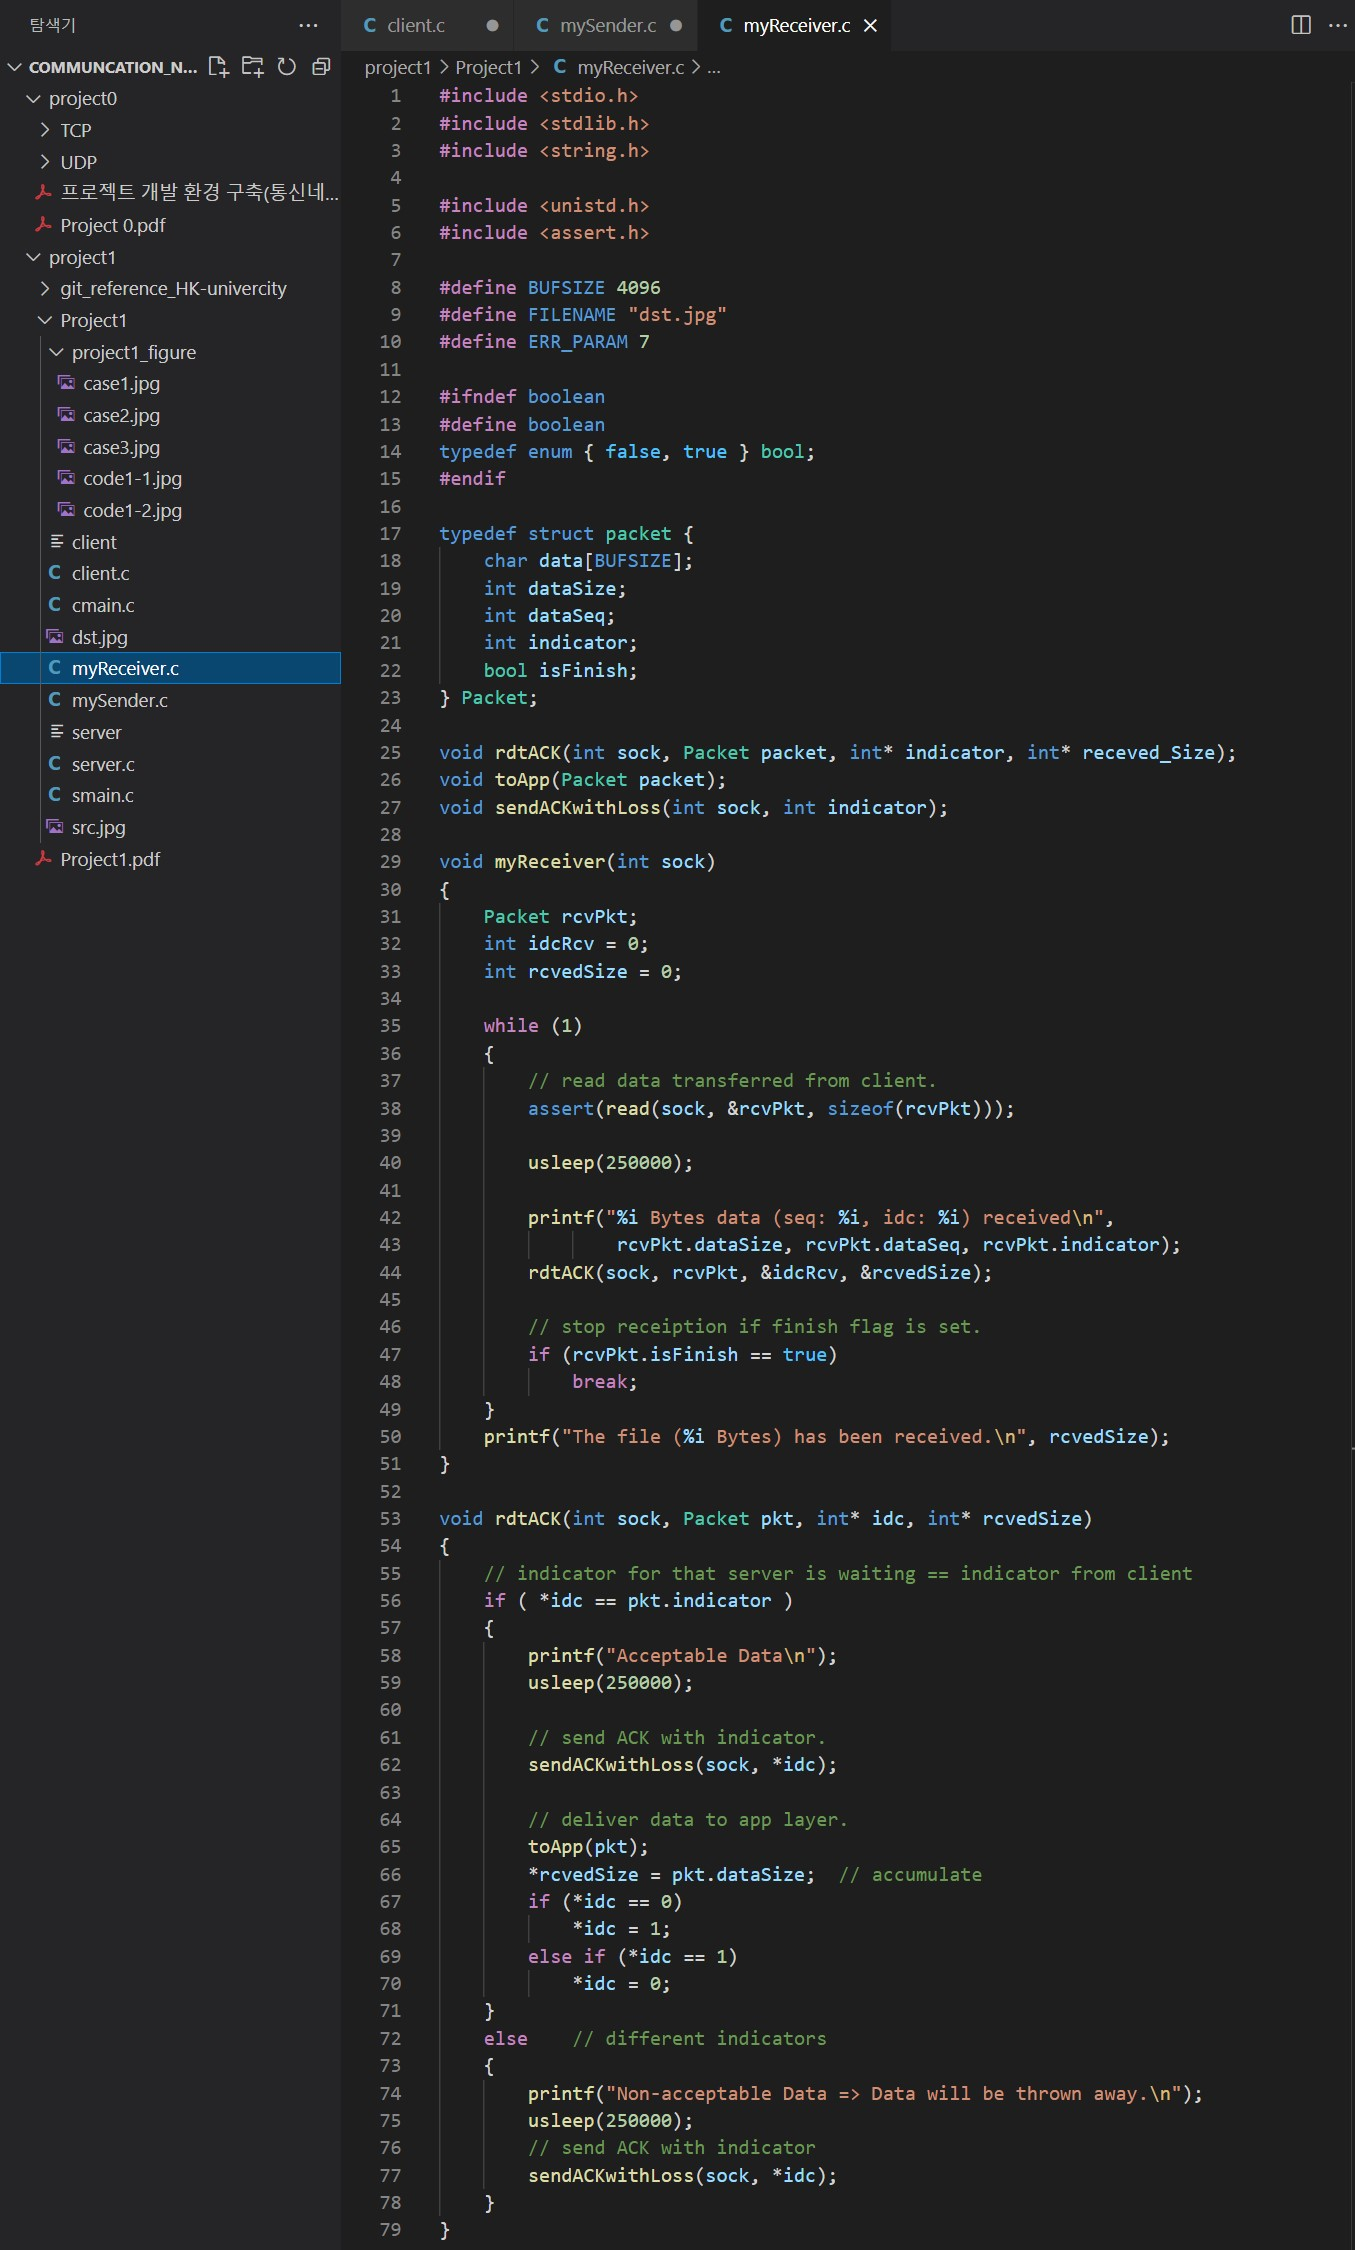
\includegraphics[width=.9\textwidth]{image/code2-1.jpg}
	\end{figure}
\vspace{-8mm}
%------------------------------------------------------------------------------------------------------------
%%%%%%%%%%%%%%%%%%%%%%%%%%%%%%%%%%%%%%%%%%%%%%%%%%%%%%%%%%%%%%%%%%%%%%%%%%%%%%%%%%%%%%%%%%%%%%%%%%%%%
\newpage
%%%%%%%%%%%%%%%%%%%%%%%%%%%%%%%%%%%%%%%%%%%%%%%%%%%%%%%%%%%%%%%%%%%%%%%%%%%%%%%%%%%%%%%%%%%%%%%%%%%%%
%------------------------------------------------------------------------------------------------------이미지
\vspace{0mm}
	\begin{figure}[!h]
		\centering
			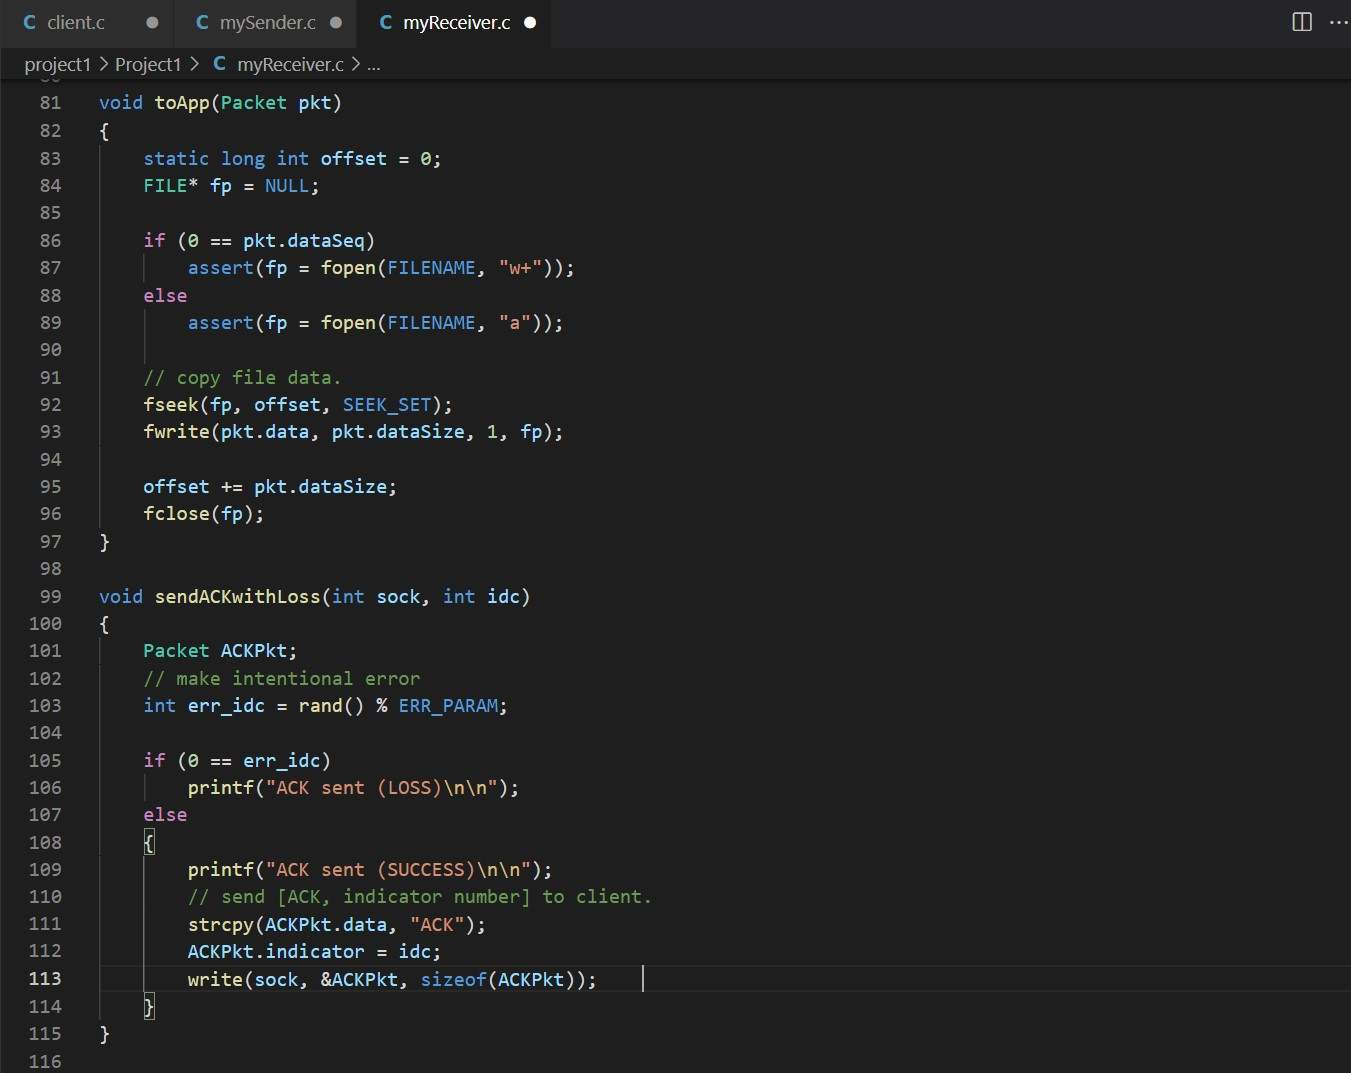
\includegraphics[width=.9\textwidth]{image/code2-2.jpg}
			\caption{rdt 3.0 TCP Server's CODE - myReceiver.c}
	\end{figure}
\vspace{-4mm}

	\section*{Terminal 프로그램 동작 Capture}
	작성한 RDT 3.0의 TCP/IP의 프로토콜이 정상적으로 packet loss가 발생하는 시나리오에서 정상적으로 작동하고 이때, 
	어떤 과정을 통해서 reliable한 data transfer를 하는지 다음의 3가지 시나리오를 통해서 확인해보고자 한다. 다음은 
	주어진 코드로 컴파일한 Client, Server를 2개의 터미널에서 동시에 실행시키면서 socket이 정상적으로 전송되어 
	dst.jpg\footnote{지난 project0와 동일}가 정상적으로 생성되는지 확인해보고자 한다.
	\vspace{-4mm}
	\subsection*{case1 : Sender에서 packet 전송성공 \& Receiver에서 Ack 전송성공}
	다음의 figure는 전송되는 37개의 packet중 sequence 0번의 packet에서의 client 와 server의 터미널 출력을 capture한 것이다. 
	Sender에서 packet의 전송을 성공하고 Receiver에서도 바로 수신을 확인하는 ACK을 바로 전송해주어, 재전송 없이 
	1회로 이루어진것을 확인할 수 있다.\\
%------------------------------------------------------------------------------------------------------이미지
\vspace{-2mm}
	\begin{figure}[!h]
		\centering
			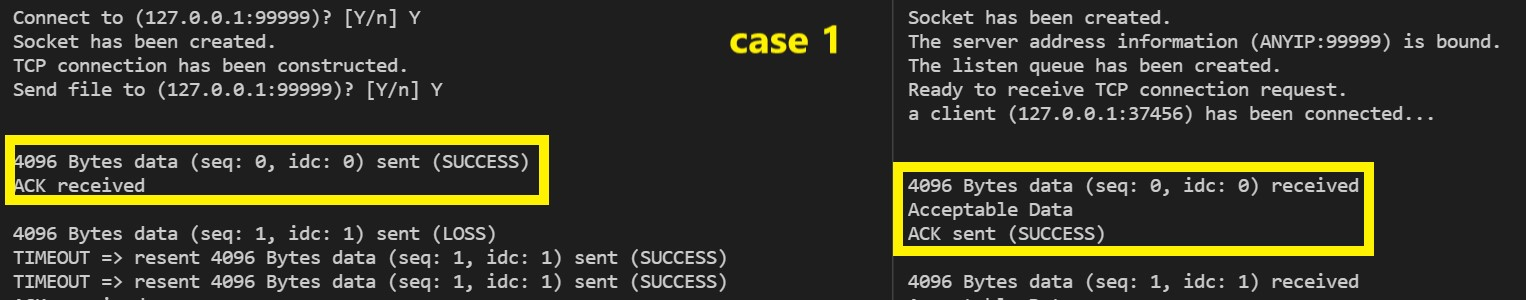
\includegraphics[width=\textwidth]{image/case1.jpg}
			\caption{case 1의 경우를 data packet중 Sequence 0에서 확인가능하다.}
	\end{figure}
\vspace{-4mm}
%------------------------------------------------------------------------------------------------------------
%%%%%%%%%%%%%%%%%%%%%%%%%%%%%%%%%%%%%%%%%%%%%%%%%%%%%%%%%%%%%%%%%%%%%%%%%%%%%%%%%%%%%%%%%%%%%%%%%%%%%
\newpage
%%%%%%%%%%%%%%%%%%%%%%%%%%%%%%%%%%%%%%%%%%%%%%%%%%%%%%%%%%%%%%%%%%%%%%%%%%%%%%%%%%%%%%%%%%%%%%%%%%%%%
	\subsection*{case 2 : Sender에서 packet 전송실패}
	Sender에서 packet의 전송을 실패하여 Receiver에서는 송신을 확인할 수 없어 ACK을 바로 전송해주지 못한다. 
	그동안 sender (client) 내부의 timer가 timeout 되게 되어 같은 sequence 14의 datapacket을 재전송하는 동작을 확인할 수 있다.\\
%------------------------------------------------------------------------------------------------------이미지
\vspace{-2mm}
	\begin{figure}[!h]
		\centering
			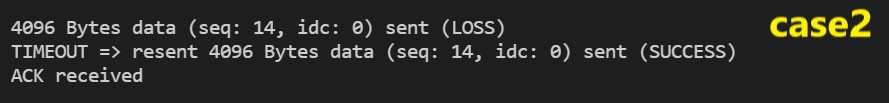
\includegraphics[width=.6\textwidth]{image/case2.jpg}
			\caption{case 2의 경우를 data packet중 Sequence 14에서 확인가능하다.}
	\end{figure}
\vspace{-8mm}
%------------------------------------------------------------------------------------------------------------
	\subsection*{case 3 : Sender에서 packet 전송성공 \& Receiver에서 Ack 전송실패}
	Sender에서 packet의 전송을 성공하여 Receiver에서도 바로 수신을 확인하는 ACK을 바로 전송해준다.
	하지만 보내는 ACK의 전송이 실패하여 Sender 입장에서는 앞서 Case 2 와 동일한 상황이라 판단해 
	다시 timeout 후 retransmission을 해준다. 하지만, 이미 sender에서는 해당 sequence의 data packet을
	정상적으로 처리하였으므로,\footnote{처리하는 과정에서 indicator를 toggle 시켜 재전송된 packet과 indicator가 달라 duplicate 된 것을 확인할 수 있다.}
	figure에서와 같이 중복된 data packet의 data를 bind 하지않고 버리는것을 확인할 수 있다. 이때 ACK은 중복으로 받은 packet의 indicator를 보내줌으로서 
	Sender 측면에서도 정상으로 전송이 된것을 확인시켜, stop and wait protocol 상에서 다음 packet을 받을 수 있도록 해준다.\\
%------------------------------------------------------------------------------------------------------이미지
\vspace{-2mm}
	\begin{figure}[!h]
		\centering
			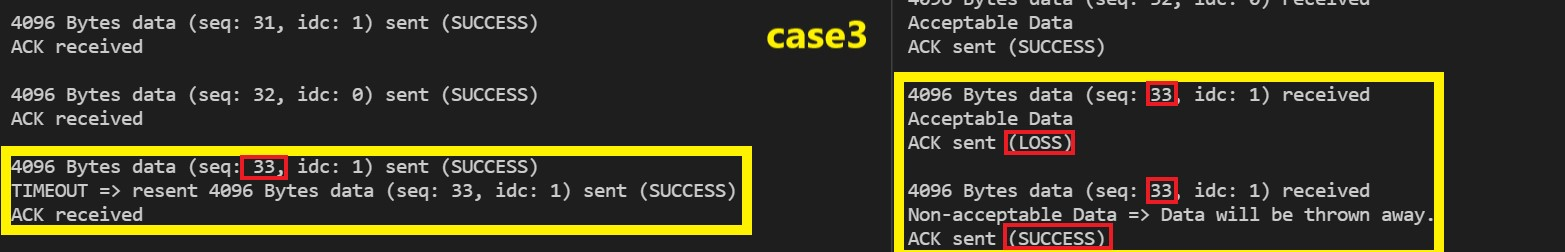
\includegraphics[width=\textwidth]{image/case3.jpg}
			\caption{case 3의 경우를 data packet중 Sequence 33에서 확인가능하다.}
	\end{figure}
\vspace{-8mm}
%------------------------------------------------------------------------------------------------------------
	\section*{Discussion}
    이번 Project를 통해서 구현해본 rdt3.0 의 TCP/IP 프로토콜의 동작을 통해서, Sender 기분에서 Data Packet을 Transmission 하는 action이 
    reliable한 데이터의 전송을 하기 위해 1개의 data packet 단위로 각각의 packet의 수신을 확인하는 receiver로 부터 ACK을 송신해야 진행되므로
    각각 Data Packet 단위에서 Stop and Wait의 동작을 진행되는것을 확인할 수 있었고, 이떄문에 코드에서 설정한 RTT를 감안한 Sleep 의 시간으로 지난 Project0와 동일한 강아지 사진을 보내는 socket 프로그램이지만 대기하는 시간으로 인해, 다른 재전송 acteion 보다 Stop and Wait 프로토콜 자체로 비효율적임을 확인해 볼 수 있었다.
    
    Reliable Data Transfer를 위해서 크게 3가지의 기능을 이용하였는데, 첫째로 Sender가 Receiver의 수신을 확인하기 위해 ACK 을 송신받는 ARQ 이다. 이 동작으로 Sender는 Data Packet을 transfer하고 ACK 을 송신을 기달리는 state로 Ttansition 하는데 이점에서, 우리가 구현한 프로토콜의 Stop and Wait를 확인할 수 있다.\\
    두번째로 Indicator\footnote{수업에서 다룬 Sequence Number}를 이용하였는데, 이는 전송되는 Data Packet의 순서가 라우팅등 네트워크 환경으로 지연되어 순서가 변하거나 기타 송신문제로 Sender에서 retransmission으로 인해 순서가 변하는 경우를 대비하기 위해 구현되었다. 앞서 우리는 Stop and Wait
    protocol을 이용하였으므로, Sender는 하나의 종류의 packet의 전송이 완료될때 다음을 전송하므로 이때 Receiver에 순서가 바뀌어 arrived할 data packet의 종류는 2가지 뿐이라, Sequence number가 아닌 간략한 
    0 또는 1의 indicator를 통해 이를 구현하였다.\\
    세번째로는 Timer 기능이다. rdt 3.0이 상정하는 packet loss가 존재하는 network 환경에서 아예 packet이 
    전송이 되지 않는경우가 있으므로 이때 하나의 data packet 단위로 전송이 완료되어야 다음 packet으로 
    넘어가는 stop and wait protocol 에서는 packet loss가 일어날 경우 TCP/IP 프로토콜이 정지할 가능성이 있다. 따라서 이를 방지하기 위해 data packet을 보내고 일정시간 이상 ack의 송신이 이루어지지 않을 경우 
    packet loss를 상정하고 retransmission을 수행하는 Timer를 구현하였다. 
    위의 3가지 요소를 이용해 stop and wait protocol 상에서 reliable data transfer를 실습해볼 수 있었고, 
    해당 프로토콜의 장단점을 확인해볼 수 있었다.
%--------------------------------------------------------------------------------------------------
